% Szkielet dla pracy inżynierskiej pisanej w języku angielskim.

\documentclass[english,bachelor,a4paper,oneside]{ppfcmthesis}

\usepackage[utf8]{inputenc}
\usepackage[OT4]{fontenc}

% Authors here.
\author{%
   Ignacy Iksiński \album{22222} \and 
   Wincent Woliński \album{22222} \and 
   Zdzisio Szmal \album{22222} \and 
   Barnaba Wojnowski \album{22222}}
\title{A Few Words About the Nature~of~Things}        % Note how we protect the final title phrase from breaking
\ppsupervisor{prof.~dr hab.~inż.~Alojzy Wołodyjowski} % Your supervisor comes here.
\ppyear{2006}                                         % Year of final submission (not graduation!)

\begin{document}

% Front matter starts here
\frontmatter\pagestyle{empty}%
\maketitle\cleardoublepage%

% Blank info page for "karta dyplomowa"
\thispagestyle{empty}\vspace*{\fill}%
\begin{center}Tutaj przychodzi karta pracy dyplomowej;\\oryginał wstawiamy do wersji dla archiwum PP, w pozostałych kopiach wstawiamy ksero.\end{center}%
\vfill\cleardoublepage%

% Table of contents.
\pagenumbering{Roman}\pagestyle{ppfcmthesis}%
\tableofcontents* \cleardoublepage%

% Main content of your thesis starts here.
\mainmatter%

\chapter{Lorem Ipsum}

\section{Lorem}

Lorem ipsum dolor sit amet, consectetuer adipiscing elit. Nunc fringilla facilisis massa. Donec
ultrices dignissim quam. Phasellus vel erat quis diam tempor porttitor. Maecenas purus ligula,
varius id, suscipit in, congue quis, erat. Vivamus erat purus, laoreet rutrum, aliquet eleifend,
porta a, erat. Etiam id neque id nunc porttitor nonummy. Mauris pulvinar mi quis elit. Sed placerat.
Cras dictum neque vel odio. Sed a augue.

Aenean eu ligula. Nulla sit amet metus et risus vehicula elementum. Vivamus a eros. Etiam lorem
odio, iaculis ac, vulputate vitae, cursus a, tortor. Sed sagittis volutpat libero. Integer ornare,
dui nec vulputate auctor, ante mi lacinia ipsum, nec mollis ipsum libero at arcu. Suspendisse ut
ligula. Nunc metus. Proin mollis pellentesque ante. Donec dictum. Sed purus ante, placerat eget,
vestibulum in, lobortis ut, pede.

Sed blandit. Fusce blandit turpis id eros auctor dictum. Ut porttitor mollis magna. Nam iaculis sem
vel velit. Sed sollicitudin libero non quam. In hac habitasse platea dictumst. Praesent tristique,
justo vitae mollis fringilla, nisl ligula feugiat lacus, ac vestibulum mi turpis in nisi. Aenean
tristique fermentum erat. Integer consectetuer erat quis ante. Morbi gravida hendrerit nulla. Etiam
magna.

\subsection{Ipsum}

Curabitur adipiscing. Nam justo quam, dapibus eu, dignissim eu, hendrerit consequat, odio. Praesent
mi ligula, vulputate et, ullamcorper ut, pellentesque ut, massa. Suspendisse potenti. Morbi interdum
nisi vel justo. Aenean in tortor id mi dapibus porttitor. Nunc convallis. Nullam vitae felis.
Maecenas fringilla, lorem quis aliquam laoreet, elit justo tincidunt nisi, ac sollicitudin sapien
nulla non nisi. Etiam et mauris. Nunc scelerisque rhoncus leo.

Morbi posuere nisi id libero. Etiam tincidunt facilisis sem. Suspendisse vulputate, lectus quis
volutpat consectetuer, urna massa vestibulum tellus, nec vehicula dolor orci id odio. Nam faucibus
sem eu nisl ullamcorper lobortis. Sed quis ipsum. Morbi volutpat pellentesque erat. Quisque ipsum
velit, aliquet eu, imperdiet ut, commodo sed, est. Proin euismod porta enim. Mauris sit amet purus.
Nunc ac turpis. Nunc tellus magna, sagittis in, pellentesque vitae, semper et, sem. Vivamus et odio.
Suspendisse tincidunt mattis leo. Morbi pharetra. Quisque fermentum, lectus eget feugiat iaculis,
enim neque accumsan felis, id hendrerit enim erat et ante. Nunc blandit commodo est. Fusce venenatis
urna quis lorem. Aenean nisi. Vivamus ornare velit in magna imperdiet dapibus.

\subsection{Aliquam Venenatis}

Cras non enim eget mi aliquam venenatis. Duis posuere imperdiet quam. Maecenas egestas. In tempus
tortor quis pede. Aenean eget mauris sit amet ipsum scelerisque porttitor. Vestibulum nisl.
Vestibulum id velit eget tellus ultrices laoreet. Sed pellentesque, odio eget adipiscing commodo,
turpis lorem placerat lacus, et interdum quam mi quis odio. Nam et magna. Pellentesque vitae nisl.
In erat est, iaculis nec, sodales imperdiet, dictum at, eros. Nullam eget leo. Praesent nunc. Morbi
id erat. Pellentesque vel felis vitae est consectetuer interdum. Fusce venenatis. Nam rhoncus tortor
et sem. Sed ut sem aliquet urna congue suscipit. Nulla eget risus in purus molestie feugiat.
Phasellus non libero vel odio vehicula placerat.

Aenean velit. Vestibulum dui sem, scelerisque non, nonummy quis, accumsan eget, ipsum. Quisque nec
est et ipsum bibendum venenatis. Donec eget pede. Sed vitae ante et metus pulvinar fermentum. Nullam
scelerisque laoreet dui. Aliquam consectetuer. Quisque molestie eros a felis. Maecenas nec nisi.
Praesent mollis nisl sit amet pede. Phasellus iaculis elementum ante.

Fusce lacinia magna ut lacus. In aliquet diam eget augue. Curabitur blandit nisi sit amet nulla.
Donec nunc. Nullam pellentesque eleifend nisi. Proin ac elit. Fusce a neque. Nunc felis. Aenean
sodales. Etiam a risus non elit commodo rhoncus. Ut mi. Cras gravida neque nec diam. Proin consequat
vestibulum nunc. Aliquam mattis justo et purus. Sed feugiat.

Fusce fermentum. Nulla orci lectus, pellentesque sit amet, egestas sed, ornare a, erat. Vivamus ante
odio, auctor ac, elementum eget, feugiat sit amet, enim. Aliquam venenatis semper erat. Pellentesque
habitant morbi tristique senectus et netus et malesuada fames ac turpis egestas. Aliquam non tellus.
Mauris ornare massa iaculis magna. Morbi eu enim. Mauris ultrices. Vivamus dapibus aliquet nulla.
Quisque consectetuer.

\section{Pellentesque Habitant}

Pellentesque est nisl, scelerisque in, dictum vel, dapibus nec, lacus. Donec eu quam sed ligula
luctus volutpat. Donec ornare ornare purus. Mauris ligula eros, pulvinar nec, viverra in, tristique
quis, nunc. Pellentesque at diam. Integer tempus risus vitae lorem. Vestibulum sed lorem id elit
convallis rutrum. Quisque lobortis massa. Pellentesque habitant morbi tristique senectus et netus et
malesuada fames ac turpis egestas. Maecenas purus. Etiam hendrerit malesuada libero. Sed non mauris.

Pellentesque habitant morbi tristique senectus et netus et malesuada fames ac turpis egestas. Sed
ligula. Quisque nec augue. Suspendisse id lacus. Mauris a turpis. Curabitur interdum nulla tempus
justo. Sed nisl mauris, volutpat eleifend, suscipit in, ornare vitae, odio. Ut tempor, pede sed
volutpat ornare, mauris elit laoreet turpis, non posuere lorem nunc eu risus. Curabitur vulputate,
risus et auctor dapibus, ipsum nisl gravida nulla, vitae venenatis nibh libero id tellus. In
accumsan aliquet augue.

In consectetuer, magna in ornare eleifend, neque leo tempor nibh, quis viverra neque sapien
malesuada orci. Quisque eget magna. Integer tempus. Sed malesuada, orci a cursus posuere, justo
magna laoreet mauris, at pulvinar sapien velit ut nisi. Sed sed augue quis libero hendrerit feugiat.
Nam porta. In et massa. Curabitur blandit purus vitae risus luctus tristique. Sed ipsum. Morbi
tincidunt, dolor ut aliquam luctus, magna libero sagittis risus, eget dignissim risus lacus quis
magna. Donec tincidunt varius elit. Ut in velit. Curabitur dui velit, vestibulum in, tristique
nonummy, venenatis et, eros. Maecenas mi leo, placerat vel, congue vitae, semper ut, nunc. Lorem
ipsum dolor sit amet, consectetuer adipiscing elit. Mauris orci elit, hendrerit vestibulum,
vulputate ut, venenatis et, mauris. Curabitur vitae tortor vitae elit vulputate congue. Mauris felis
dui, lobortis vel, consectetuer id, cursus at, sapien.

Integer ut turpis. Duis odio ligula, lobortis ut, egestas a, porttitor id, ligula. Nunc vulputate,
ipsum quis varius aliquet, est eros sagittis urna, interdum imperdiet lorem ipsum tincidunt nibh.
Vivamus dictum porttitor diam. Lorem ipsum dolor sit amet, consectetuer adipiscing elit. Praesent at
nulla. Praesent tincidunt ipsum a velit. Fusce ut ipsum sed purus scelerisque nonummy. Cras
imperdiet velit eu nibh. Ut ultrices mauris et risus.




% All appendices and extra material, if you have any.
\cleardoublepage\appendix%
%\chapter{Załączniki}

\section{Definicje XMLSchema dla modeli}
\subsection{Model bazy danych}
\begin{Verbatim}
<?xml version="1.0" encoding="UTF-8"?>
<xsd:schema xmlns:xsd="http://www.w3.org/2001/XMLSchema"
	xmlns:tns="http://www.jdbmeasure.org/database-model"
	targetNamespace="http://www.jdbmeasure.org/database-model"
	xmlns="http://www.jdbmeasure.org/database-model"
	elementFormDefault="qualified">
	<xsd:complexType name="tcolumn">
		<xsd:attribute name="name" type="xsd:string" use="required" />
		<xsd:attribute name="type" type="xsd:string" use="required" />
		<xsd:attribute name="is_nullable" type="xsd:boolean" />
		<xsd:attribute name="is_id" type="xsd:boolean" />
		<xsd:attribute name="min_value" type="xsd:string" />
		<xsd:attribute name="max_value" type="xsd:string" />
		<xsd:attribute name="is_lob" type="xsd:boolean" />
		<xsd:attribute name="is_unique" type="xsd:boolean" />
		<xsd:attribute name="unique_group_id" type="xsd:string" />
	</xsd:complexType>
	<xsd:complexType name="treference">
		<xsd:attribute name="column_name" 
			type="xsd:string" use="required" />
		<xsd:attribute name="relation_name" 
			type="xsd:string" use="required" />
		<xsd:attribute name="relation_column_name" 
			type="xsd:string" use="required" />
	</xsd:complexType>
	<xsd:complexType name="tcolumns">
		<xsd:sequence minOccurs="0" maxOccurs="unbounded">
			<xsd:element name="column" type="tns:tcolumn" />
		</xsd:sequence>
	</xsd:complexType>
	<xsd:complexType name="treferences">
		<xsd:sequence minOccurs="0" maxOccurs="unbounded">
			<xsd:element name="reference" type="tns:treference" />
		</xsd:sequence>
	</xsd:complexType>
	<xsd:complexType name="trelation">
		<xsd:sequence minOccurs="0">
			<xsd:element name="columns" type="tns:tcolumns" />
			<xsd:element name="references" type="tns:treferences" minOccurs="0" />
		</xsd:sequence>
		<xsd:attribute name="name" type="xsd:string" use="required" />
	</xsd:complexType>
	<xsd:complexType name="trelations">
		<xsd:sequence minOccurs="0" maxOccurs="unbounded">
			<xsd:element name="relation" type="tns:trelation" />
		</xsd:sequence>
	</xsd:complexType>
	<xsd:complexType name="trelation-population">
		<xsd:attribute name="relation_name" type="xsd:string" use="required" />
		<xsd:attribute name="expression" type="xsd:string" use="required" />
	</xsd:complexType>
	<xsd:complexType name="tpopulation">
		<xsd:sequence minOccurs="0" maxOccurs="unbounded">
			<xsd:element name="relation-population" 
				type="tns:trelation-population" />
		</xsd:sequence>
	</xsd:complexType>
	<xsd:complexType name="tdatabase-model">
		<xsd:sequence minOccurs="0">
			<xsd:element name="relations" type="tns:trelations" />
			<xsd:element name="population" type="tns:tpopulation" />
			<xsd:element name="model-description" type="xsd:string" />
		</xsd:sequence>
	</xsd:complexType>
	<xsd:element name="database-model" type="tns:tdatabase-model" />
</xsd:schema>
\end{Verbatim}

\subsection{Model obciążenia}
\begin{Verbatim}
<?xml version="1.0" encoding="UTF-8"?>
<xsd:schema xmlns="http://www.jdbmeasure.org/load-model"
	xmlns:tns="http://www.jdbmeasure.org/load-model"
	xmlns:xsd="http://www.w3.org/2001/XMLSchema"
	elementFormDefault="qualified"
	targetNamespace="http://www.jdbmeasure.org/load-model">
	<xsd:complexType name="tparameter">
		<xsd:attribute name="number" type="xsd:double" use="required" />
		<xsd:attribute name="type" type="xsd:string" use="required" />
		<xsd:attribute name="is_nullable" type="xsd:boolean" />
		<xsd:attribute name="is_id" type="xsd:boolean" />
		<xsd:attribute name="min_value" type="xsd:string" />
		<xsd:attribute name="max_value" type="xsd:string" />
		<xsd:attribute name="is_lob" type="xsd:boolean" />
		<xsd:attribute name="is_unique" type="xsd:boolean" />
		<xsd:attribute name="unique_group_id" type="xsd:string" />
		<xsd:attribute name="ref_relation_name" type="xsd:string" />
		<xsd:attribute name="ref_relation_column_name" type="xsd:string" />
	</xsd:complexType>
	<xsd:complexType name="tparameters">
		<xsd:sequence minOccurs="0" maxOccurs="unbounded">
			<xsd:element name="parameter" type="tns:tparameter" />
		</xsd:sequence>
	</xsd:complexType>
	<xsd:complexType name="toperation">
		<xsd:sequence minOccurs="1" maxOccurs="unbounded">
			<xsd:element name="definition" type="xsd:string" />
			<xsd:element name="parameters" type="tns:tparameters" />
			<xsd:element name="operation-description" type="xsd:string" />
		</xsd:sequence>
		<xsd:attribute name="name" type="xsd:string" use="required" />
		<xsd:attribute name="type" type="xsd:string" use="required" />
	</xsd:complexType>
	<xsd:complexType name="toperations">
		<xsd:sequence minOccurs="0" maxOccurs="unbounded">
			<xsd:element name="operation" type="tns:toperation" />
		</xsd:sequence>
	</xsd:complexType>
	<xsd:complexType name="ttransaction-operation">
		<xsd:attribute name="operation_name" type="xsd:string" 
			use="required" />
		<xsd:attribute name="number" type="xsd:integer" />
	</xsd:complexType>
	<xsd:complexType name="ttransaction-operations">
		<xsd:sequence minOccurs="0" maxOccurs="unbounded">
			<xsd:element name="transaction-operation" 
				type="tns:ttransaction-operation" />
		</xsd:sequence>
	</xsd:complexType>
	<xsd:complexType name="ttransaction">
		<xsd:sequence minOccurs="0">
			<xsd:element name="transaction-operations" 
				type="tns:ttransaction-operations" />
			<xsd:element name="transaction-description" 
				type="xsd:string" />
		</xsd:sequence>
		<xsd:attribute name="name" type="xsd:string" use="required" />
	</xsd:complexType>
	<xsd:complexType name="ttransactions">
		<xsd:sequence minOccurs="0" maxOccurs="unbounded">
			<xsd:element name="transaction" type="tns:ttransaction" />
		</xsd:sequence>
	</xsd:complexType>
	<xsd:complexType name="tactor-transaction">
		<xsd:attribute name="transaction_name" type="xsd:string" 
			use="required" />
		<xsd:attribute name="avg_call_number" type="xsd:integer" 
			use="required" />
	</xsd:complexType>
	<xsd:complexType name="tactor-transactions">
		<xsd:sequence minOccurs="0" maxOccurs="unbounded">
			<xsd:element name="actor-transaction" 
				type="tns:tactor-transaction" />
		</xsd:sequence>
	</xsd:complexType>
	<xsd:complexType name="tactor">
		<xsd:sequence minOccurs="0">
			<xsd:element name="actor-transactions" 
				type="tns:tactor-transactions" />
			<xsd:element name="actor-description" type="xsd:string" />
		</xsd:sequence>
		<xsd:attribute name="name" type="xsd:string" use="required" />
		<xsd:attribute name="session_length" type="xsd:string" use="required" />
		<xsd:attribute name="min_number" type="xsd:string" use="required" />
		<xsd:attribute name="max_number" type="xsd:string" use="required" />
		<xsd:attribute name="parent" type="xsd:string" />
		<xsd:attribute name="inh_level" type="xsd:double" />
	</xsd:complexType>
	<xsd:complexType name="tactors">
		<xsd:sequence minOccurs="0" maxOccurs="unbounded">
			<xsd:element name="actor" type="tns:tactor" />
		</xsd:sequence>
	</xsd:complexType>
	<xsd:complexType name="tload-model">
		<xsd:sequence minOccurs="0">
			<xsd:element name="operations" type="tns:toperations" />
			<xsd:element name="transactions" type="tns:ttransactions" />
			<xsd:element name="actors" type="tns:tactors" />
			<xsd:element name="description" type="xsd:string" />
		</xsd:sequence>
	</xsd:complexType>
	<xsd:element name="load-model" type="tns:tload-model" />
</xsd:schema>
\end{Verbatim}

\subsection{Model testu}
\begin{Verbatim}
<?xml version="1.0" encoding="UTF-8"?>
<xsd:schema xmlns="http://www.jdbmeasure.org/load-model"
	xmlns:tns="http://www.jdbmeasure.org/load-model"
	xmlns:xsd="http://www.w3.org/2001/XMLSchema"
	elementFormDefault="qualified"
	targetNamespace="http://www.jdbmeasure.org/test-model">
	<xsd:complexType name="tproperty">
		<xsd:attribute name="name" type="xsd:string" />
		<xsd:attribute name="value" type="xsd:string" />
	</xsd:complexType>
	<xsd:complexType name="tjdbc-connection-properties">
		<xsd:sequence minOccurs="6" maxOccurs="6">
			<xsd:element name="property" type="tns:tproperty" />
		</xsd:sequence>
	</xsd:complexType>
	<xsd:complexType name="ttest-model">
		<xsd:sequence minOccurs="1" maxOccurs="1">
			<xsd:element name="jdbc-connection-properties" 
			type="tns:tjdbc-connection-properties" />
		</xsd:sequence>
		<xsd:attribute name="delete_db_after_test" type="xsd:boolean" use="required" />
		<xsd:attribute name="rte_number" type="xsd:integer" use="required" />
		<xsd:attribute name="c" type="xsd:string" use="required" />
		<xsd:attribute name="n" type="xsd:string" use="required" />
		<xsd:attribute name="a" type="xsd:string" use="required" />
	</xsd:complexType>
	<xsd:element name="test-model" type="tns:ttest-model" />
	</xsd:schema>
\end{Verbatim}
	
\section{Przykładowy raport}\label{sect:raportexample}

Poniżej został zamieszczony przykładowy raport w formie tekstowej:\\
\begin{Verbatim}
*********************************************************************************
*                   Test Result Analyze (Date: June 19, 2006)                   *
*********************************************************************************

Total test number:       19
Test operation number:   9
Test transaction number: 10
RTE number:              8

*********************************************************************************
*                             Load test operations                              *
*********************************************************************************
Operation name: DELETE FROM TBL_PRODUCT
Operation type: DELETE
Operation definition:  DELETE FROM TBL_PRODUCT WHERE PRODUCT_ID = ?
Operation description: Usunięcie produktu

Number of test operations per RTE:  2
Total number of test operations:    16

Avarage RTE time:               2s 85ms 61us
Median RTE time:                2s 90ms 362us
Standard deviation RTE time:    24ms 226us

Single operation time avarage:  1s 42ms 530us
*********************************************************************************
Operation name: UPDATE TBL_CUSTOMER
Operation type: UPDATE
Operation definition: UPDATE TBL_CUSTOMER SET PASSWORD = ?, FIRSTNAME = ?, SURNAME = ?, 
                      DATE_OF_BIRTH = ?, SEX = ?, IS_SINGLE = ? WHERE LOGIN = ?
Operation description: Edycja danych osoby

Number of test operations per RTE:  25
Total number of test operations:    200

Avarage RTE time:               9s 380ms 75us
Median RTE time:                9s 271ms 203us
Standard deviation RTE time:    239ms 620us

Single operation time avarage:  375ms 203us
*********************************************************************************
Operation name: INSERT INTO TBL_PRODUCT
Operation type: INSERT
Operation definition: INSERT INTO TBL_PRODUCT(PRODUCT_ID,CATEGORY_ID,NAME,DESCRIPTION,
                      PRICE,PICTURE) VALUES(?,?,?,?,?,?)
Operation description: Wstawienie nowego produktu

Number of test operations per RTE:  5
Total number of test operations:    40

Avarage RTE time:               1s 395ms 474us
Median RTE time:                1s 430ms 633us
Standard deviation RTE time:    136ms 733us

Single operation time avarage:  279ms 94us
*********************************************************************************
Operation name: UPDATE TBL_PRODUCT
Operation type: UPDATE
Operation definition: UPDATE TBL_PRODUCT SET CATEGORY_ID = ?,NAME = ?,
                      DESCRIPTION = ?,PRICE = ?,PICTURE = ? WHERE PRODUCT_ID = ?
Operation description: Edycja produktu

Number of test operations per RTE:  5
Total number of test operations:    40

Avarage RTE time:               1s 113ms 84us
Median RTE time:                1s 132ms 911us
Standard deviation RTE time:    61ms 696us

Single operation time avarage:  222ms 616us
*********************************************************************************
Operation name: INSERT INTO TBL_ORDER
Operation type: INSERT
Operation definition: INSERT INTO TBL_ORDER(ORDER_ID,CUSTOMER_ID,DATE_OF_ORDERED) 
                      VALUES(?,?,?)
Operation description: Wstawienie nowego zamówienia

Number of test operations per RTE:  25
Total number of test operations:    200

Avarage RTE time:               5s 441ms 257us
Median RTE time:                5s 408ms 721us
Standard deviation RTE time:    117ms 831us

Single operation time avarage:  217ms 650us
*********************************************************************************
Operation name: SELECT FROM TBL_CUSTOMER
Operation type: SELECT
Operation definition:  SELECT PASSWORD FROM TBL_CUSTOMER WHERE LOGIN = ?
Operation description: Sprawdzenie uprawnień osoby do systemu

Number of test operations per RTE:  25
Total number of test operations:    200

Avarage RTE time:               3s 931ms 560us
Median RTE time:                3s 996ms 802us
Standard deviation RTE time:    434ms 464us

Single operation time avarage:  157ms 262us
*********************************************************************************
Operation name: INSERT INTO TBL_ORDER_ITEM
Operation type: INSERT
Operation definition: INSERT INTO TBL_ORDER_ITEM(ORDER_ID,PRODUCT_ID,
                      NUMBER_OF_ELEMENTS,TOTAL_PRICE) VALUES(?,?,?,?)
Operation description: Wstawienie nowego elementu do zamówienia

Number of test operations per RTE:  100
Total number of test operations:    800

Avarage RTE time:               13s 868ms 642us
Median RTE time:                13s 870ms 341us
Standard deviation RTE time:    205ms 197us

Single operation time avarage:  138ms 686us
*********************************************************************************
Operation name: INSERT INTO TBL_SUBSCRIBER
Operation type: INSERT
Operation definition:  INSERT INTO TBL_SUBSCRIBER(EMAIL) VALUES(?)
Operation description: Dodanie osoby do listy subskrybentów

Number of test operations per RTE:  147
Total number of test operations:    1176

Avarage RTE time:               19s 945ms 149us
Median RTE time:                19s 982ms 314us
Standard deviation RTE time:    239ms 890us

Single operation time avarage:  135ms 681us
*********************************************************************************
Operation name: SELECT FROM TBL_PRODUCT
Operation type: SELECT
Operation definition: SELECT * FROM TBL_PRODUCT WHERE PRICE >= ? AND PRICE <= ? 
                      AND CATEGORY_ID = ?
Operation description: Wyszukiwanie produktów po cenie i kategorii

Number of test operations per RTE:  5162
Total number of test operations:    41296

Avarage RTE time:               22s 18ms 457us
Median RTE time:                25s 53ms 151us
Standard deviation RTE time:    6s 550ms 933us

Single operation time avarage:  4ms 265us
*********************************************************************************


*********************************************************************************
*                           Load test transactions                              *
*********************************************************************************
Transaction name:        Delete product
Transaction description: Usunięcie produktu

Number of test transactions per RTE:  20
Total number of test transactions:    160

Avarage RTE time:                 6s 38ms 369us
Median RTE time:                  6s 46ms 971us
Standard deviation RTE time:      75ms 397us

Single transaction time avarage:  301ms 918us
*********************************************************************************
Transaction name:        Create order
Transaction description: Uwtorzenie zamówienia

Number of test transactions per RTE:  200
Total number of test transactions:    1600

Avarage RTE time:                 37s 678ms 386us
Median RTE time:                  37s 740ms 455us
Standard deviation RTE time:      554ms 157us

Single transaction time avarage:  188ms 391us
*********************************************************************************
Transaction name:        Add product
Transaction description: Dodanie produktu

Number of test transactions per RTE:  40
Total number of test transactions:    320

Avarage RTE time:                 5s 441ms 764us
Median RTE time:                  5s 474ms 878us
Standard deviation RTE time:      90ms 172us

Single transaction time avarage:  136ms 44us
*********************************************************************************
Transaction name:        Edit product
Transaction description: Edycja produktu

Number of test transactions per RTE:  40
Total number of test transactions:    320

Avarage RTE time:                 5s 287ms 651us
Median RTE time:                  5s 288ms 301us
Standard deviation RTE time:      48ms 131us

Single transaction time avarage:  132ms 191us
*********************************************************************************
Transaction name:        Edit account
Transaction description: Edycja konta użytkownika

Number of test transactions per RTE:  200
Total number of test transactions:    1600

Avarage RTE time:                 24s 727ms 572us
Median RTE time:                  24s 660ms 541us
Standard deviation RTE time:      277ms 206us

Single transaction time avarage:  123ms 637us
*********************************************************************************
Transaction name:        Add to subscriber list
Transaction description: Dodanie do listy subskrybentów

Number of test transactions per RTE:  1180
Total number of test transactions:    9440

Avarage RTE time:                 124s 487ms 60us
Median RTE time:                  125s 56ms 664us
Standard deviation RTE time:      1s 347ms 541us

Single transaction time avarage:  105ms 497us
*********************************************************************************
Transaction name:        Login/Logout
Transaction description: Sprawdzenie uprawnień

Number of test transactions per RTE:  200
Total number of test transactions:    1600

Avarage RTE time:                 2s 375ms 948us
Median RTE time:                  2s 445ms 641us
Standard deviation RTE time:      257ms 584us

Single transaction time avarage:  11ms 879us
*********************************************************************************
Transaction name:        Compare products
Transaction description: Porównanie produktów

Number of test transactions per RTE:  5900
Total number of test transactions:    47200

Avarage RTE time:                 53s 662ms 378us
Median RTE time:                  56s 6ms 419us
Standard deviation RTE time:      6s 911ms 264us

Single transaction time avarage:  9ms 95us
*********************************************************************************
Transaction name:        Find product
Transaction description: Wyszukanie produktu

Number of test transactions per RTE:  11800
Total number of test transactions:    94400

Avarage RTE time:                 37s 15ms 272us
Median RTE time:                  42s 768ms 436us
Standard deviation RTE time:      7s 750ms 387us

Single transaction time avarage:  3ms 136us
*********************************************************************************
Transaction name:        Show product
Transaction description: Wyświetlenie informacji o produkcie

Number of test transactions per RTE:  11800
Total number of test transactions:    94400

Avarage RTE time:                 35s 627ms 102us
Median RTE time:                  36s 740ms 291us
Standard deviation RTE time:      4s 81ms 466us

Single transaction time avarage:  3ms 19us
*********************************************************************************


*********************************************************************************
*                         Proportion test operations                            *
*********************************************************************************
Operation name: DELETE FROM TBL_PRODUCT
Operation type: DELETE
Operation definition:  DELETE FROM TBL_PRODUCT WHERE PRODUCT_ID = ?
Operation description: Usunięcie produktu

Number of test operations per RTE:  2
Total number of test operations:    16

Avarage RTE time:               393ms 264us
Median RTE time:                363ms 636us
Standard deviation RTE time:    263ms 988us

Best RTE time:                 69ms 416us
Worst RTE time:                1s 15ms 137us
*********************************************************************************
Operation name: UPDATE TBL_CUSTOMER
Operation type: UPDATE
Operation definition: UPDATE TBL_CUSTOMER SET PASSWORD = ?, FIRSTNAME = ?, SURNAME = ?, 
                      DATE_OF_BIRTH = ?, SEX = ?, IS_SINGLE = ? WHERE LOGIN = ?
Operation description: Edycja danych osoby

Number of test operations per RTE:  25
Total number of test operations:    200

Avarage RTE time:               295ms 41us
Median RTE time:                209ms 466us
Standard deviation RTE time:    296ms 921us

Best RTE time:                   44ms 540us
Worst RTE time:              1s 584ms 139us
*********************************************************************************
Operation name: UPDATE TBL_PRODUCT
Operation type: UPDATE
Operation definition: UPDATE TBL_PRODUCT SET CATEGORY_ID = ?,NAME = ?,DESCRIPTION = ?,
                      PRICE = ?,PICTURE = ? WHERE PRODUCT_ID = ?
Operation description: Edycja produktu

Number of test operations per RTE:  5
Total number of test operations:    40

Avarage RTE time:               207ms 163us
Median RTE time:                154ms 801us
Standard deviation RTE time:    228ms 696us

Best RTE time:                 2ms 472us
Worst RTE time:                990ms 713us
*********************************************************************************
Operation name: INSERT INTO TBL_PRODUCT
Operation type: INSERT
Operation definition: INSERT INTO TBL_PRODUCT(PRODUCT_ID,CATEGORY_ID,NAME,DESCRIPTION,
		      PRICE,PICTURE) VALUES(?,?,?,?,?,?)
Operation description: Wstawienie nowego produktu

Number of test operations per RTE:  5
Total number of test operations:    40

Avarage RTE time:               205ms 368us
Median RTE time:                162ms 464us
Standard deviation RTE time:    170ms 302us

Best RTE time:                41ms 399us
Worst RTE time:               1s 23ms 814us
*********************************************************************************
Operation name: INSERT INTO TBL_ORDER_ITEM
Operation type: INSERT
Operation definition: INSERT INTO TBL_ORDER_ITEM(ORDER_ID,PRODUCT_ID,
                      NUMBER_OF_ELEMENTS,TOTAL_PRICE) VALUES(?,?,?,?)
Operation description: Wstawienie nowego elementu do zamówienia

Number of test operations per RTE:  100
Total number of test operations:    800

Avarage RTE time:               186ms 632us
Median RTE time:                137ms 882us
Standard deviation RTE time:    190ms 189us

Best RTE time:                37ms 657us
Worst RTE time:                1s 613ms 920us
*********************************************************************************
Operation name: INSERT INTO TBL_ORDER
Operation type: INSERT
Operation definition: INSERT INTO TBL_ORDER(ORDER_ID,CUSTOMER_ID,DATE_OF_ORDERED) 
		      VALUES(?,?,?)
Operation description: Wstawienie nowego zamówienia

Number of test operations per RTE:  25
Total number of test operations:    200

Avarage RTE time:               180ms 410us
Median RTE time:                140ms 853us
Standard deviation RTE time:    170ms 383us

Best RTE time:                   43ms 836us
Worst RTE time:                1s 342ms 889us
*********************************************************************************
Operation name: INSERT INTO TBL_SUBSCRIBER
Operation type: INSERT
Operation definition:  INSERT INTO TBL_SUBSCRIBER(EMAIL) VALUES(?)
Operation description: Dodanie osoby do listy subskrybentów

Number of test operations per RTE:  147
Total number of test operations:    1176

Avarage RTE time:               158ms 349us
Median RTE time:                122ms 477us
Standard deviation RTE time:    133ms 441us

Best RTE time:                37ms 528us
Worst RTE time:                1s 536ms 946us
*********************************************************************************
Operation name: SELECT FROM TBL_CUSTOMER
Operation type: SELECT
Operation definition:  SELECT PASSWORD FROM TBL_CUSTOMER WHERE LOGIN = ?
Operation description: Sprawdzenie uprawnień osoby do systemu

Number of test operations per RTE:  25
Total number of test operations:    200

Avarage RTE time:               61ms 229us
Median RTE time:                34ms 54us
Standard deviation RTE time:    147ms 123us

Best RTE time:                324us
Worst RTE time:                1s 167ms 411us
*********************************************************************************
Operation name: SELECT FROM TBL_PRODUCT
Operation type: SELECT
Operation definition: SELECT * FROM TBL_PRODUCT WHERE PRICE >= ? AND PRICE <= ? 
                      AND CATEGORY_ID = ?
Operation description: Wyszukiwanie produktów po cenie i kategorii

Number of test operations per RTE:  5162
Total number of test operations:    41296

Avarage RTE time:               2ms 890us
Median RTE time:                1ms 357us
Standard deviation RTE time:    13ms 344us

Best RTE time:                239us
Worst RTE time:                923ms 227us
*********************************************************************************


*********************************************************************************
*                          Proportion test transactions                         *
*********************************************************************************
Transaction name:        Delete product
Transaction description: Usunięcie produktu

Number of test transactions per RTE:  20
Total number of test transactions:    160

Avarage RTE time:                 655ms 63us
Median RTE time:                  464ms 114us
Standard deviation RTE time:      563ms 622us

Best RTE time:                78ms 685us
Worst RTE time:                3s 30ms 686us
*********************************************************************************
Transaction name:        Create order
Transaction description: Uwtorzenie zamówienia

Number of test transactions per RTE:  200
Total number of test transactions:    1600

Avarage RTE time:                 328ms 103us
Median RTE time:                  237ms 514us
Standard deviation RTE time:      312ms 69us

Best RTE time:                39ms 886us
Worst RTE time:                2s 381ms 393us
*********************************************************************************
Transaction name:        Edit account
Transaction description: Edycja konta użytkownika

Number of test transactions per RTE:  200
Total number of test transactions:    1600

Avarage RTE time:                 305ms 930us
Median RTE time:                  224ms 440us
Standard deviation RTE time:      277ms 284us

Best RTE time:                45ms 801us
Worst RTE time:                2s 339ms 871us
*********************************************************************************
Transaction name:        Add product
Transaction description: Dodanie produktu

Number of test transactions per RTE:  40
Total number of test transactions:    320

Avarage RTE time:                 210ms 980us
Median RTE time:                  150ms 292us
Standard deviation RTE time:      198ms 471us

Best RTE time:                39ms 878us
Worst RTE time:                1s 567ms 57us
*********************************************************************************
Transaction name:        Edit product
Transaction description: Edycja produktu

Number of test transactions per RTE:  40
Total number of test transactions:    320

Avarage RTE time:                 197ms 779us
Median RTE time:                  151ms 103us
Standard deviation RTE time:      223ms 225us

Best RTE time:                1ms 649us
Worst RTE time:                1s 231ms 649us
*********************************************************************************
Transaction name:        Add to subscriber list
Transaction description: Dodanie do listy subskrybentów

Number of test transactions per RTE:  1180
Total number of test transactions:    9440

Avarage RTE time:                 190ms 601us
Median RTE time:                  142ms 517us
Standard deviation RTE time:      173ms 312us

Best RTE time:                26ms 208us
Worst RTE time:                1s 999ms 356us
*********************************************************************************
Transaction name:        Login/Logout
Transaction description: Sprawdzenie uprawnień

Number of test transactions per RTE:  200
Total number of test transactions:    1600

Avarage RTE time:                 71ms 324us
Median RTE time:                  31ms 42us
Standard deviation RTE time:      185ms 929us

Best RTE time:                312us
Worst RTE time:                1s 627ms 652us
*********************************************************************************
Transaction name:        Compare products
Transaction description: Porównanie produktów

Number of test transactions per RTE:  5900
Total number of test transactions:    47200

Avarage RTE time:                 6ms 797us
Median RTE time:                  4ms 218us
Standard deviation RTE time:      17ms 169us

Best RTE time:                704us
Worst RTE time:                936ms 129us
*********************************************************************************
Transaction name:        Find product
Transaction description: Wyszukanie produktu

Number of test transactions per RTE:  11800
Total number of test transactions:    94400

Avarage RTE time:                 2ms 862us
Median RTE time:                  1ms 271us
Standard deviation RTE time:      16ms 568us

Best RTE time:                243us
Worst RTE time:                985ms 474us
*********************************************************************************
Transaction name:        Show product
Transaction description: Wyświetlenie informacji o produkcie

Number of test transactions per RTE:  11800
Total number of test transactions:    94400

Avarage RTE time:                 2ms 777us
Median RTE time:                  1ms 277us
Standard deviation RTE time:      13ms 635us

Best RTE time:                241us
Worst RTE time:                975ms 861us
*********************************************************************************
\end{Verbatim}

\section{Tabele wyników testów}
Poniżej przedstawiono tabele (tab.~\ref{tab:time_tab01}, \ref{tab:time_tab02}, 
\ref{tab:time_tab03}, \ref{tab:time_tab04}) z~przykładowymi wynikami pomiarów 
dla rozdziału \ref{chap:test_bench}.

\begin{table}[h]
\begin{center}
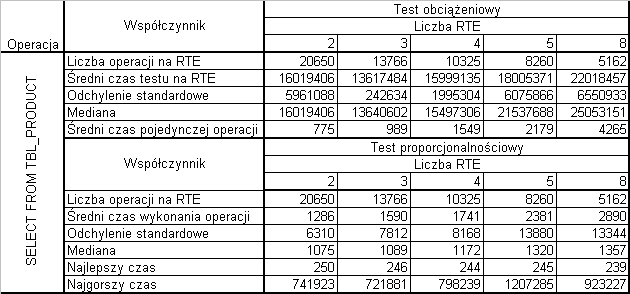
\includegraphics[width=0.9\linewidth]{figures/time_tab01.png}
\end{center}
\caption{Czasy wykonania operacji selekcji produktu}\label{tab:time_tab01}
\end{table}

\begin{table}[h]
\begin{center}
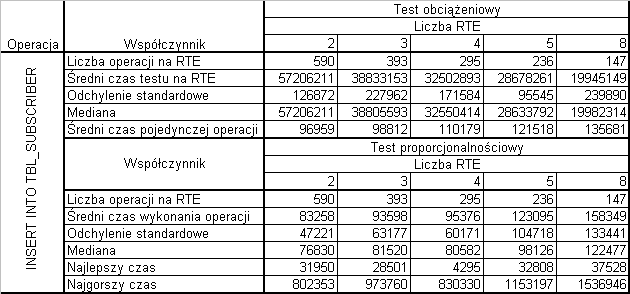
\includegraphics[width=0.9\linewidth]{figures/time_tab02.png}
\end{center}
\caption{Czasy wykonania operacji wstawienia osoby do listy subskrybcji}\label{tab:time_tab02}
\end{table}

\begin{table}[h]
\begin{center}
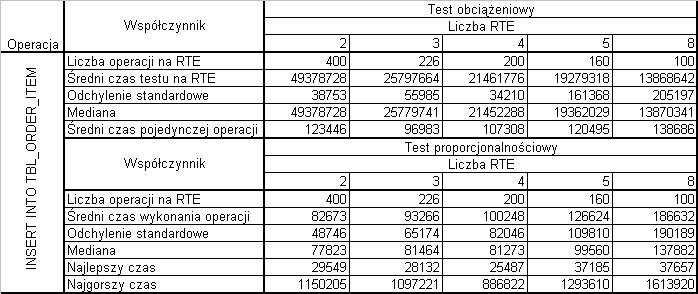
\includegraphics[width=0.9\linewidth]{figures/time_tab03.png}
\end{center}
\caption{Czasy wykonania operacji dodania produktu do zamówienia}\label{tab:time_tab03}
\end{table}

\begin{table}[h]
\begin{center}
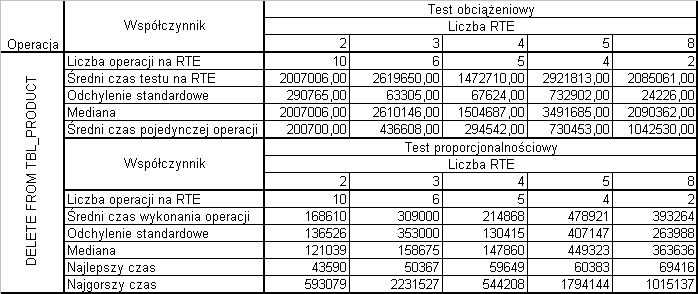
\includegraphics[width=0.9\linewidth]{figures/time_tab04.png}
\end{center}
\caption{Czasy wykonania operacji usunięcia produktu}\label{tab:time_tab04}
\end{table}



% Bibliography (books, articles) starts here.
\bibliographystyle{alpha}{\raggedright\sloppy\small\bibliography{bibliography}}

% Colophon is a place where you should let others know about copyrights etc.
\ppcolophon

\end{document}
